%Struktur
% -Festlegung von Software-Kriterien
% -Auswahl des Verfahrens
% -Reproduktion des Verfahrens aus der Literatur
% 	-Kantenerkennung
% 	-Segmentierung
%	-Probleme & besondere Erkenntnisse
% -Erweiterung des Verfahrens
%	-Grundlegende Änderungen des Verfahrens
%	-False edge removal
%	-Point marking and cloud filtering
%	-misc.


\chapter{Methodik} \label{Methodik}
Dieses Kapitel beschäftigt sich mit der genauen Methodik zur Aufstellung eines Verfahrens für die Kantenerkennung und Segmentierung in wachsenden Punktwolken. Es werden in diesem Kapitel zwei Themen behandelt: die Reproduktion des gewählten Verfahrens aus der Literatur und seine Erweiterung mit weiteren Funktionalitäten. 

\section{Implementierung des Verfahrens}
Bevor das Verfahren für den Online-Erkennung angepasst wird, soll es zuerst zwecks einer Überprüfung unverändert implementiert werden. Somit soll sichergestellt werden, dass das Verfahren funktioniert und erweiterbar ist. Da die Autoren das Quellcode des Verfahrens nicht öffentlich zugängig gemacht haben, muss das Programm reproduziert werden. Die Reproduktion des Programms erfolgt in zwei Schritten. Als erstes wird das Verfahrens zur Kantenerkennung reproduziert und danach das Verfahren zur Kantensegmentierung. Obwohl andere Skriptsprachen wie Python und MATLAB hinsichtlich des Prototypings Vorteile anbieten, wird das Programm zwecks der besseren Leistungsfähigkeit der Sprache in C++ implementiert \autocite{svensson_performance_2021}. Viele Funktionalitäten der PCL-Bibliothek \autocite{rusu_3d_2011} werden auch für den Entwurf des Verfahrens verwendet.

\begin{figure}[h]
	\includegraphics[scale=0.12]{Abbildungen/ablauf_plan_edge.png}
	\centering
	\caption[Programmablaufplan zur Kantenerkennung]{Das Programmablaufplan zur Erkennung Randpunkte \autocite{ni_edge_2016}.}
	\label{flow_chart}
\end{figure}

\subsection{Verfahren zur Kantenerkennung} \label{edge_detection_reprod}
Während Randelemente in zweidimensionale Bilder eine klare Definition haben, werden diese Randelemente und Kanten für 3D-Punktwolken nicht einheitlich definiert. Es lässt sich erkennen, dass Kanten einer dreidimensionalen Punktwolke aus Randpunkten bestehen. In diesem Verfahren werden die geometrischen Eigenschaften einer Kollektion von Punkten zur Erkennung Randpunkte berücksichtigt. Randpunkte weisen diese besondere geometrische Eigenschaft auf \textendash{} der Winkelabstand zwischen benachbarten Randpunkte ist im Vergleich zu anderen benachbarten Punkten deutlich größer. Kantungen stellen den Grenzbereich zwischen zwei angrenzenden Ebenen dar, deren Normale in unterschiedlichen Richtungen zeigen. Diese geometrischen Eigenschaften werden zur Erkennung von Randpunkten verwendet. \autocite[1-2]{ni_edge_2016}

Im folgenden wird die Kantenerkennung detaillierter erläutert, welches ein Teilverfahren des AGPN-Verfahrens ist. Zwecks der Übersichtlichkeit wird dieses Teilverfahren als \textit{\hyperref[alg:find_edge_points]{FindEdgePoints}} referiert. Für einen Punkt~\textit{o} wird eine Sammlung von \textit{K\textsubscript{1}} benachbarten Punkten mittels eines kd-Baums erstellt. Diese Sammlung wird als eine Nachbarschaft \textit{N\textsubscript{o}} referiert. Danach wird mittels eines RANSAC-Algorithmus eine Ebene~\textit{E\textsubscript{N\textsubscript{o}}} auf diese Nachbarschaft gefittet, um Ausreißer herauszufiltern und zwei angrenzenden Flächen innerhalb der Nachbarschaft voneinander zu trennen. Danach wird Überprüft, ober der Punkt \textit{o} auf der Ebene \textit{E\textsubscript{N\textsubscript{o}}} liegt. Falls dieser Punkt ein Ausreißer der Ebene \textit{E\textsubscript{N\textsubscript{o}}} ist, kann er keinen Randpunkt sein und das Verfahren wird für einen neuen Punkt wiederholt. Ansonsten wird in den nächsten Schritt des \textit{\hyperref[alg:find_edge_points]{FindEdgePoints}} Verfahrens gelangt. Abbildung~\ref{RANSAC-Ebene} visualisiert die Trennung zwischen unterschiedlichen Flächen einer Punktwolke mittels des RANSAC-Verfahrens. 

\begin{figure}[h]
	\includegraphics[width=\textwidth]{Abbildungen/RANSAC-Ebene.png}
	\centering
	\caption[Trennung mehrerer Ebenen mit RANSAC]{Eine lokale Ebene (rot dargestellt) neben anderen Oberflächen (blau dargestellt). In \textbf{(a)} sind drei Ebenen zu sehen, wobei in \textbf{(b)} nur zwei zu sehen sind. \autocite{ni_edge_2016}}
	\label{RANSAC-Ebene}
\end{figure} 

Im Falle, dass der Punkt \textit{o} ein Inlier ist und zu der Ebene \textit{E\textsubscript{N\textsubscript{o}}} gehört, fängt die Überprüfung der geometrischen Eigenschaften der Nachbarschaft \textit{N\textsubscript{o}} an. Um die Ebene von \textit{E\textsubscript{N\textsubscript{o}}} näherungsweise zu schätzen, wird zuerst die Normale \textit{$\vec{n\textsubscript{o}}$} der Ebene geschätzt. Mit den Inliers zu der Ebene~\textit{E\textsubscript{N\textsubscript{o}}} wird auch die Gleichung dieser Ebene näherungsweise zurückgegeben. Diese Gleichung wird weiterhin optimiert und daraus die Normale \textit{$\vec{n\textsubscript{o}}$} ermittelt, indem das RANSAC-Verfahren wiederholt wird. Danach erfolgt die Errechnung des Winkelabstands zwischen den jeweiligen Nachbarpunkte in \textit{N\textsubscript{o}}. Hierfür wird für die Ebene \textit{E\textsubscript{N\textsubscript{o}}} die jeweiligen Eigenvektoren $\vec{u}$ und $\vec{v}$ aus der Normale $\vec{n\textsubscript{o}}$ errechnet. Es gibt ein vorhandenes Verfahren von PCL zur Ausrechnung der Eigenvektoren, allerdings stehen diese nicht genau orthogonal zu einander. Stattdessen werden zur Ermittelung \textit{$\vec{u}$} zwei zufällig gewählte Punkten aus der Inliers verwendet. Es wird dabei sichergestellt, dass keiner der Punkten der Punkt \textit{o} sind. Zur Errechnung des Winkelabstands werden zuerst die Winkel aller Punkte der lokalen Ebene \textit{E\textsubscript{N\textsubscript{o}}} errechnet. Mit dem Punkt \textit{o} als Ursprung wird für jeden Punkt \textit{p\textsubscript{i}}, aus allen Inliers, der Winkel \textit{$\theta_i$} zu dem Eigenvektor~$\vec{v}$ errechnet. Danach wird die Differenz zwischen zwei konsekutiver Punktwinkel~$\theta_i$ und $\theta_{i+1}$ errechnet, welcher den Winkelabstand \textit{G\textsubscript{$\theta$}} zwischen zwei Punkten - \textit{p\textsubscript{i}} und \textit{p\textsubscript{i+1}} - beträgt. Bei einem Winkelabstand größer als einem bestimmten Schwellenwert $\alpha$ wird der Punkt \textit{o} als ein Randpunkt markiert. Ni, Lin et al. verwenden einen Schwellenwert $\alpha$ von $\frac{\pi}{2}$. Abbildung~\ref{edge_boundary} zeigt, wie der Winkelabstand zwischen Punkten am Rand der Punktwolke aussieht.

\begin{figure}[t]
	\includegraphics[width=0.5\textwidth]{Abbildungen/angular_gap_boundary}
	\centering
	\caption[Visualisierung des Winkelabstandes zwischen Punkten]{Der Winkelabstand \textit{G\textsubscript{$\theta$}} zwischen Punkten am Rand der Punktwolke. \textbf{(a)} zeigt einen internen Punkt \textit{o} und ein Nachbarpunkt \textit{p\textsubscript{i}}. Im Vergleich dazu zeigt \textbf{(b)} \textit{o} am Rand und den großen Winkelabstand \textit{G\textsubscript{$\theta$}} zwischen Punkte \textit{p\textsubscript{i}} und \textit{p\textsubscript{i + 1}}. \autocite{ni_edge_2016}}
	\label{edge_boundary}
\end{figure}

\begin{figure}[!b]
	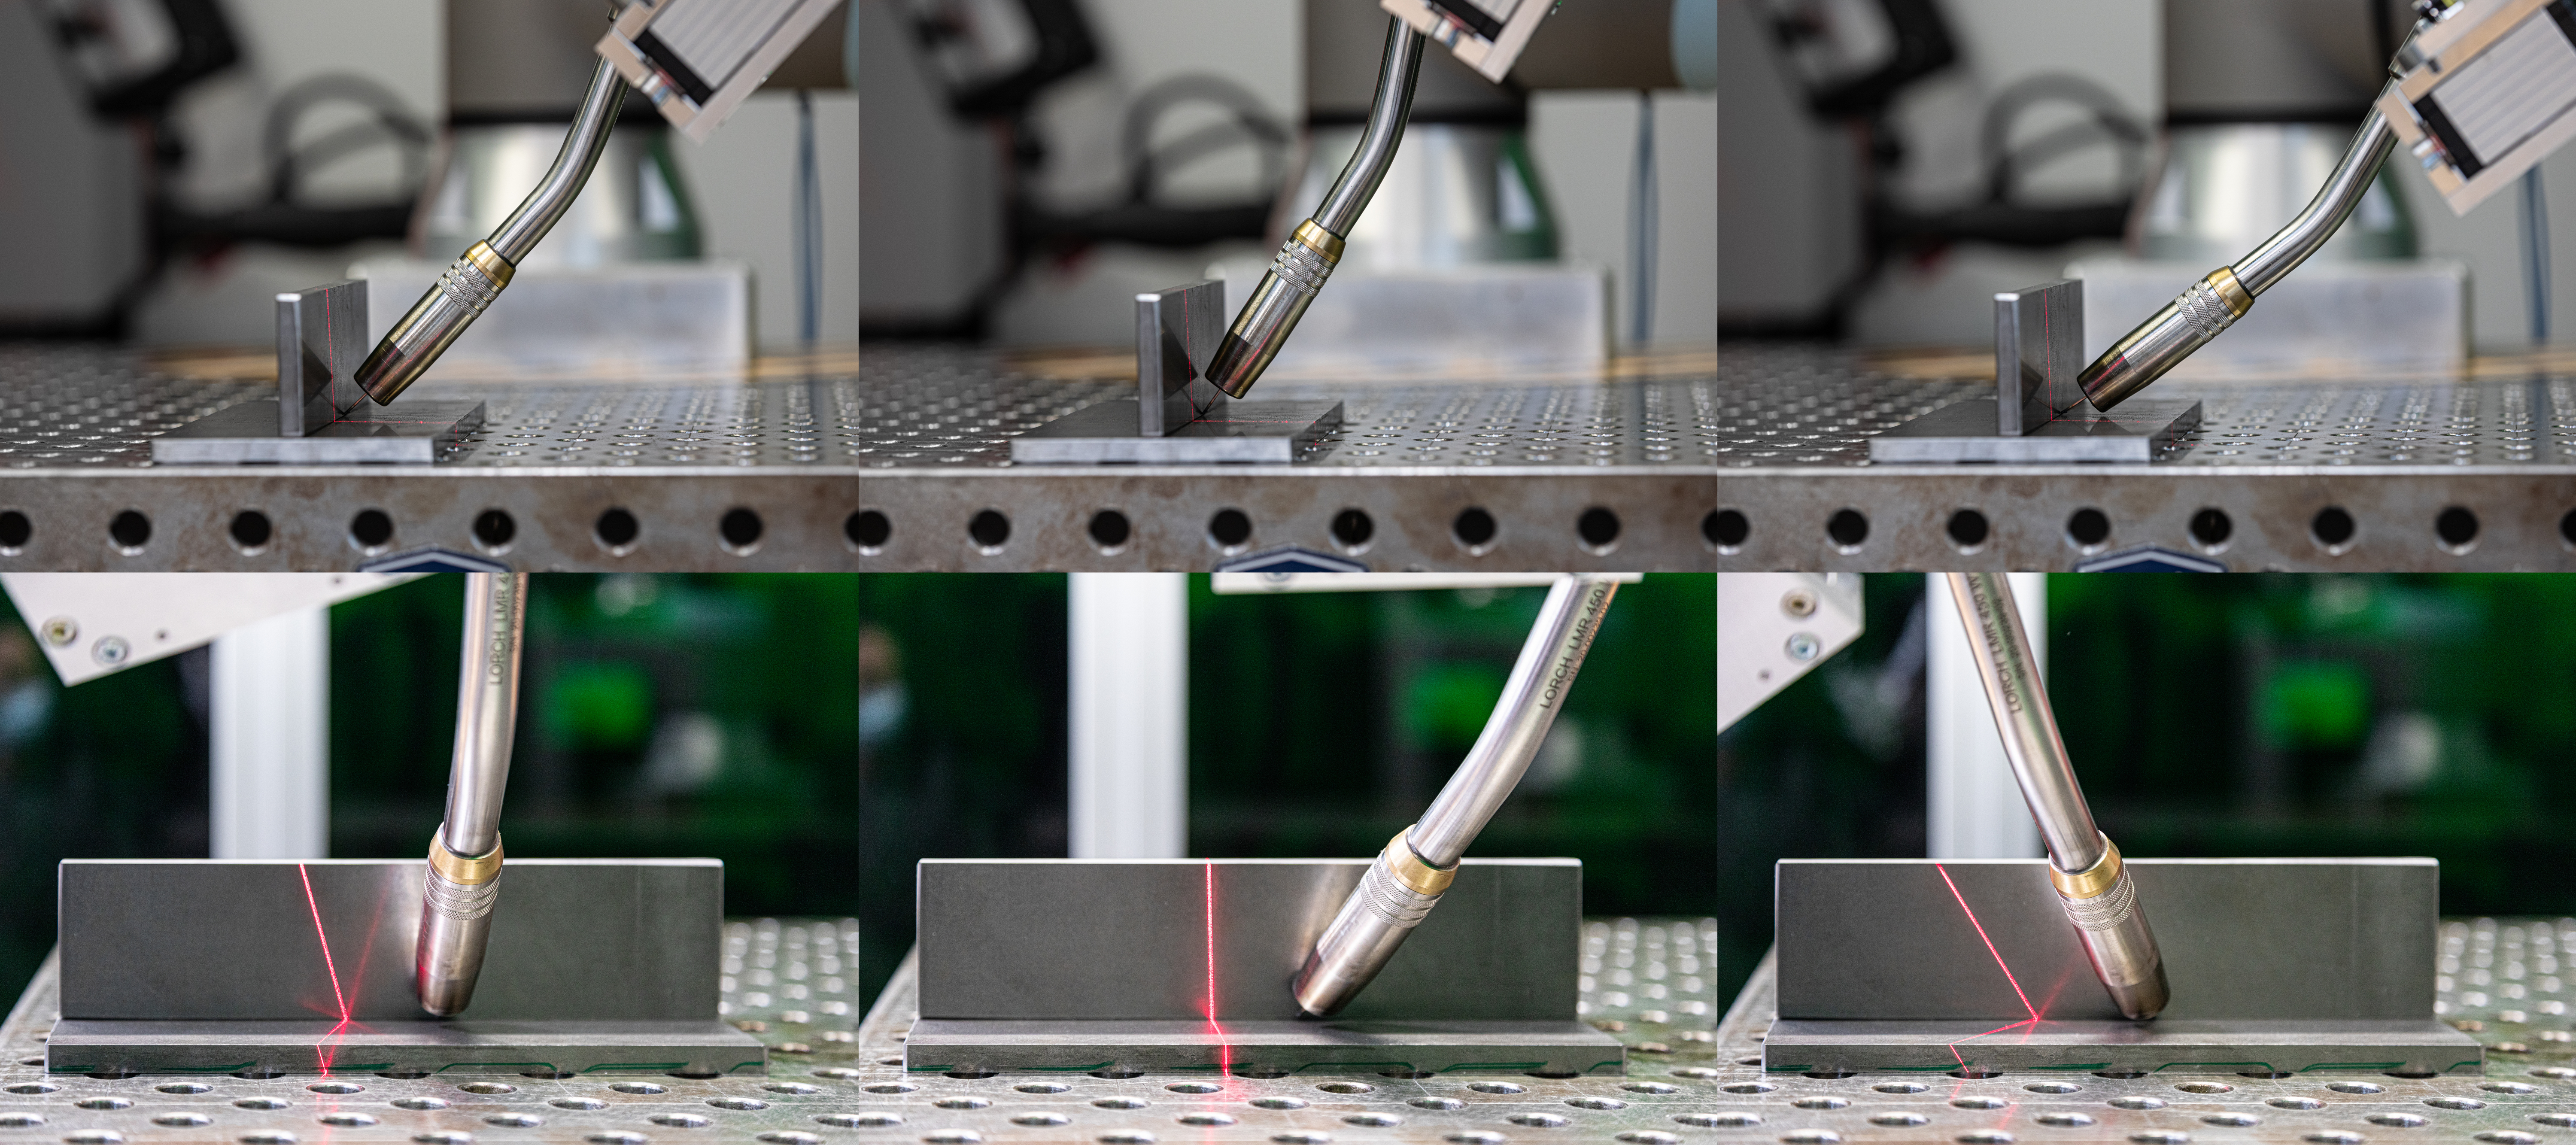
\includegraphics[width = 0.8\textwidth]{Abbildungen/collage.jpg}
	\centering
	\caption[Innenkante zweier Blechen]{Die Kegelnaht zweier Blechen ist eine Innenkante}
	\label{fig: Innenkante}
\end{figure}

Auch die Erkennung von Punkten in Innen- und Außenkanten ist durch diese Berechnungen möglich. Abbildung~\ref{fig: Innenkante} zeigt eine Innenkante von zwei Blechen, die zum Schweißnaht wird. Wie bereits erwähnt, wird eine Punktwolke mit zwei angrenzenden Flächen mittels das RANSAC-Verfahren segmentiert. Falls der Punkt \textit{o} auf der Schnittlinie beider Flächen sowie auf der lokalen Ebene \textit{E\textsubscript{N\textsubscript{o}}} liegt, dann gehört es zum lokalen Rand der Ebene. Falls der Punkt \textit{o} auf der Schnittlinie beider Flächen liegt, aber nicht zur \textit{E\textsubscript{N\textsubscript{o}}} gehört, wird er automatisch als kein Randpunkt vermerkt. Die Abbildung~\ref{edge_fold} zeigt, wie der Winkelabstand zwischen Punkten auf einer Schnittlinie zwischen zwei Flächen der Punktwolke aussieht. Die Errechnungen des Winkelabstands erfolgt nach den Gleichungen~\ref{first_equation} -~\ref{last_equation}.


\begin{equation}
\label{first_equation}
d_i^u = \overrightarrow{{op}_i} \cdot \vec{u}
\end{equation}
\begin{equation}
d_i^v = \overrightarrow{{op}_i} \cdot \vec{v}
\end{equation}
\begin{equation}
\theta_i = \arctan{\frac{d_i^u}{d_i^v}}
\end{equation}
\begin{equation}
G_\theta = \max(\theta_{i + 1} - \theta_i), i \in \{1, \ldots, N_r - 1\},
\label{last_equation}
\end{equation}

\begin{figure}[!b]
	\includegraphics[width=\textwidth]{Abbildungen/angular_gap_fold}
	\centering
	\caption[Winkelabstand zwischen Punkten zwei angrenzenden Ebenen]{Der Winkelabstand zwischen Punkten auf einer Schnittlinie zwei angrenzender Flächen. \textbf{\(a\)} zeigt ein interner Punkt \textit{o} der RANSAC-Ebene. \textbf{\(b\)} zeigt \textit{o} am lokalen Rand der RANSAC-Ebene und den Winkelabstand \textit{G\textsubscript{$\theta$}} zwischen Punkte \textit{p\textsubscript{i}} und \textit{p\textsubscript{i + 1}}. \textbf{\(c\)} zeigt \textit{o} als ein Ausreißer der RANSAC-Ebene. \autocite{ni_edge_2016}}
	\label{edge_fold}
\end{figure}

Um die Genauigkeit des Verfahrens zu versichern und die Rechenarbeit des Verfahrens zu verringern, werden gezielt zwei zusätzliche Schritte vor dem Erkennungsverfahren eingeführt. Um die Anzahl der Punkte in der Punktwolke zu verringern, wird ein Voxel-Grid basiertes Downsampling-Verfahren implementiert, um die Punktdichte der Punktwolke künstlich anzupassen und den Abstand zwischen Punkten zu vereinheitlichen. Hierzu dient die PCL-Funktion \textit{UniformSampling} verwendet \autocite{noauthor_point_2023}. Um Ausreißer aus der Punktwolke zu entfernen, wird ein statistisches Verfahren der PCL-Bibliothek namens \textit{StatisticalOutlierRemoval} zur Entfernung von Ausreißer verwendet \autocite{rusu_towards_2008}. Zur Korrekten Ausrechnung des maximalen Winkelabstands einer Nachbarschaft \textit{G\textsubscript{$\theta$}} ist eine aufsteigende Sortierung der Winkel \textit{$\theta_i$} notwendig. Diese Sortierung entspricht eine Sortierung der Punkte \textit{p\textsubscript{i}} nach ihrer aufsteigenden polaren Entfernung von dem Vektor $\vec{v}$. Die Abbildung ~\ref{vector_graph} dient zur Visualisierung der Methode zur Ausrechnung von $\theta_i$. Die Eigenvektoren $\vec{u}$ und $\vec{v}$ bilden das zweidimensionale Koordinatensystem, wobei $\vec{v}$ analog zu einer Abszisse agierte. Die Skalarprodukte \textit{d\textsubscript{i}\textsuperscript{u}} und \textit{d\textsubscript{i}\textsuperscript{v}} repräsentieren die parallelen Anteile des Vektors $\vec{{op}_i}$ der jeweiligen Eigenvektoren $\vec{u}$ und $\vec{v}$. Somit lässt sich der Winkel $\theta_i$ eines Punktes \textit{p\textsubscript{i}} zu dem Vektor $\vec{v}$ errechnen. Abbildung~\ref{edge_points_table} zeigt all erkannten Kanten einer eines Schreibtisches und dient bestätigt, dass die Kantenerkennung des AGPN-Verfahrens erwartungsgemäß funktioniert.

\begin{figure}[h]
	\includegraphics[scale=0.7]{Abbildungen/vector_graph.png}
	\centering
	\caption[Berechnung des Winkels zwischen Punkte]{Graphische Visualisierung der Berechnung des Winkels $\theta_i$}
	\label{vector_graph}
\end{figure}

\begin{figure}[h]
	\includegraphics[scale=0.37]{Abbildungen/table_edge_overlay.png}
	\centering
	\caption[Randpunkte eines Tisches]{Randpunkte eines Tisches. Die braune Punkte bilden die Ränder bzw. Kanten ab, die in der blauen Punktwolke durch das Verfahren erkannt werden}
	\label{edge_points_table}
\end{figure}

Das \textit{\hyperref[alg:find_edge_points]{FindEdgePoints}} Verfahren soll möglichst schnell erfolgen, um für den Einsatz in der Schweißrobotik geeignet zu sein. Durch die Implementierung des Programms in C++ erfolgt die Erkennung von Kanten schneller im Vergleich zu anderen Sprachen wie Python oder MATLAB. Allerdings wird die Leistungsfähigkeit moderner Rechner und CPUs durch das Programm nicht völlig ausgeschöpft. Moderne Mehrkernprozessoren bieten die Funktionalität an, Aufgaben parallel auszuführen. Isolierte Rechenaufgaben, die möglichst homogen bleiben und wiederholt werden, lassen sich sehr gut parallelisieren. Das \textit{\hyperref[alg:find_edge_points]{FindEdgePoints}} Verfahren schleift durch alle Punkte der Punktwolke durch, um Randpunkte zu erkennen. Diese Schleife eignet sich besonders zur Parallelisierung. Die Programmierschnittstelle OpenMP bietet über Compiler-Befehle die Möglichkeit an, Prozesse in C, C++ und Fortran zu parallelisieren. Das Schleifenelement des Verfahrens kann mittels OpenMP parallelisiert werden, da die Festlegung eines Punktes zum Randpunkt keinen Einfluss auf die Erkennung anderer Randpunkte hat, und somit eine isolierte Aufgabe darstellt. Es soll auch sichergestellt werden, dass eine Variable in einer Speicheradresse nicht gleichzeitig durch zwei oder mehrere parallele Instanzen der Schleife überschrieben wird. Auch Datenstrukturen sollen sorgfältig nach ihrer Eignung zur Parallelisierung gewählt werden, um Speicherlecks zu vermeiden. Auch die Berechnung des Winkels $\theta_i$ für jeden Punkt der RANSAC-Ebene \textit{E\textsubscript{N}} könnte parallelisiert werden. Eine solche Parallelisierung bringt eine deutliche Leistungssteigerung mit. 

Zusammenfassend wird für jeden Punkt \textit{o} aus der Punktwolke eine RANSAC-Ebene \textit{E\textsubscript{N\textsubscript{o}}} aus einer lokalen Nachbarschaften des Punktes mit \textit{K\textsubscript{1}} Punkten erstellt. Falls \textit{o} auf der Ebene liegt, und der größte Winkelabstand zwischen Punkten der Ebene mit Ursprung \textit{o} größer als $\alpha$ beträgt, wird \textit{o} als ein Randpunkt markiert und gespeichert. Durch die Wiederholung dieser Schritte für alle Punkte können alle Randpunkte und somit aller Kanten der Punktwolke identifiziert werden. Abbildung~\ref{flow_chart} stellt den gesamten Programmablaufplan für dieses Verfahren dar. Die Probleme bei der Reproduktion dieses Verfahrens werden im Abschnitt~\ref{Erkenntnisse} besprochen. Der detaillierter Verlauf des Verfahrens ist im Anhang~\ref{Algorithmen} als Algorithmus~\ref{alg:find_edge_points} zu finden.


\subsection{Verfahren zur Kantensegmentierung} \label{edge_segmentation}
Nachdem die Kanten der Punktwolke erkannt werden, folgt ihrer Segmentierung. Zwecks der Übersichtlichkeit wird das Verfahren zur Kantensegmentierung als \textit{SegmentEdges} benannt. Hierbei werden alle Kanten zusammen gruppiert, die ein geometrisches Merkmal des gescannten Objektes abbilden. Hierfür wird ein Region-Growing Verfahren verwendet. Punkte werden auf Basis zweier Kriterien segmentiert. Das erste Kriterium besagt, dass nur Punkte, die nah aneinander legen, einen Cluster bilden können. Das zweite Kriterium besagt, dass nur Punkte, die in einer ähnlichen Hauptrichtung zeigen, zusammen geclustert werden dürfen. Die Segmentierung erfolgt hauptsächlich in zwei Schritten - die Erstellung und Verfeinerung von Nachbarschaften sowie die Region-Growing Segmentierung der Kanten \autocite{ni_edge_2016}. Das Teilverfahren \textit{SegmentEdges} besteht aus zwei weiteren Teilverfahren - \textit{\hyperref[alg:compute_vectors]{ComputeVectors}} und \textit{\hyperref[alg:apply_region_growing]{ApplyRegionGrowing}}

Bei \textit{\hyperref[alg:compute_vectors]{ComputeVectors}} handelt es sich um die Berechnung der Richtungsvektoren und die Bestimmung der exakten Nachbarpunkte jedes Randpunktes aller Kanten. Für einen Randpunkt \textit{p\textsubscript{r}} werden eine Anzahl \textit{K\textsubscript{2}} Nachbarpunkte aus den, nach \textit{\hyperref[alg:find_edge_points]{FindEdgePoints}} erkannten Randpunkten, gesucht. Diese Sammlung wird als die Nachbarschaft \textit{N\textsubscript{p}} referenziert. Danach wird eine Linie \textit{L\textsubscript{N\textsubscript{p}}} mittels eines RANSAC-Verfahrens auf die Nachbarschaft \textit{N\textsubscript{p}} angebracht, um alle Punkte zu finden, die in der gleichen Hauptrichtung zeigten. Falls der Randpunkt \textit{p\textsubscript{r}} nicht zu den Inliers der RANSAC-Linie gehört, wird die Linie \textit{L\textsubscript{N\textsubscript{p}}} iterativ so lange angepasst, bis \textit{p\textsubscript{r}} zu den Inliers von \textit{L\textsubscript{N\textsubscript{p}}} gehört. Danach werden alle Inliers der Linie \textit{L\textsubscript{N\textsubscript{p}}} als die exakten Nachbarpunkte des Punktes \textit{p} gespeichert. Der aus \textit{L\textsubscript{N\textsubscript{p}}} ermittelte Richtungsvektor wird dem Punkt \textit{p\textsubscript{r}} zugeordnet. Dieses Verfahren wird für jeden Randpunkt wiederholt. Dieses Verfahren wird ausführlich im Anhang~\ref{Algorithmen} unter Algorithmus~\ref{alg:compute_vectors} abgebildet.

Bei \textit{\hyperref[alg:apply_region_growing]{ApplyRegionGrowing}} handelt es sich um die Implementierung des Region-Growing-Algorithmus. Hierfür wird das Region-Growing Verfahren der PCL-Bibliothek adaptiert \autocite{rusu_3d_2011}. Zuerst werden alle Punkte mit dem Label \textit{-1} markiert, um diese als \textit{unsegmentiert} zu kennzeichnen. Das Referenzwerk deutet auf die Irreversibilität des Verfahrens hin, weswegen die Auswahl eines guten Startpunktes sehr wichtig ist. Randpunkte mit einer hohen Anzahl von exakten Nachbarn können mit einer höheren Wahrscheinlichkeit eine Kante oder ein geometrisches Merkmal abbilden. Deswegen sollen alle Randpunkte nach einer absteigenden Anzahl von Nachbarpunkte sortiert werden, sodass die Auswahl eines guten Startpunktes gewährleistet wird. Für den Zuwachs eines Segments \textit{C} wird ein initialer Seedpunkt \textit{s\textsubscript{i}} gewählt, welcher im Falle des ersten Segments der Startpunkt ist. Für jeden unmarkierten (durch \textit{-1} gekennzeichnet) exakten Nachbarpunkt \textit{n\textsubscript{s}} von \textit{s} wird geprüft, ob dessen Hauptrichtungsvektor mit dem des Seedpunktes näherungsweise übereinstimmt. Dies erfolgt durch die Berechnung des Winkelabstands zwischen beiden Hauptrichtungsvektoren, der nicht einen Schwellwert, den sogenannten Glättungsfaktor $\phi$ nicht übersteigen darf. Falls der Richtungsvektor des Nachbarpunktes mit dem des Seedpunktes übereinstimmt, wird es dem Segment \textit{C} hinzugefügt und mit dem Index des Segments markiert. Danach wird \textit{n\textsubscript{s}} zu einer Queue voller neuen Seedpunkte \textit{s\textsubscript{c}} hinzugefügt, die für den weiteren Zuwachs des Segments \textit{C} verwendet werden. Nachdem alle exakte Nachbarpunkte von \textit{s\textsubscript{i}} markiert werden, wird dieser Schritt für alle neue \textit{s\textsubscript{c}} wiederholt, bis kein Punkt mit dem Richtungsvektor von \textit{s\textsubscript{i}} übereinstimmt. Diese Schleife soll zwecks der Wiederverwendbarkeit in einer separaten Methode namens \textit{\hyperref[alg:grow_segment]{GrowSegment}} gekapselt werden. Danach wird ein neuer unmarkierter initialer Seedpunkt \textit{s\textsubscript{i}} gewählt und das ganze Verfahren wiederholt. Im Algorithmen~\ref{Algorithmen} wird das Verfahren ausführlicher beschreibt. Die Abbildung~\ref{segments_table} zeigt alle Segmente in unterschiedlichen Farben an, die durch Region-Growing Verfahren aus den Kanten des Tisches erkannt werden. Das \textit{\hyperref[alg:grow_segment]{GrowSegment}} sowie \textit{\hyperref[alg:apply_region_growing]{ApplyRegionGrowing}} Verfahren werden ausführlich im Anhang~\ref{Algorithmen} unter Algorithmus~\ref{alg:grow_segment} beziehungsweise Algorithmus~\ref{alg:apply_region_growing} behandelt.¸

\begin{figure}[h]
	\includegraphics[width=\textwidth]{Abbildungen/table_segments.png}
	\centering
	\caption[Segmente eines Tisches]{Die, durch das AGPN-Verfahren erkannten Segmenten des Tisches aus Abbildung~\ref{edge_points_table}.}
	\label{segments_table}
\end{figure}

%Nachdem die Funktionsweise des AGPNs getestet wurde, erfolgte die Erweiterung des Verfahrens, um die Kantenerkennung und Segmentierung für wachsenden Punktwolken zu ermöglichen.

\section{Erweiterung des Verfahrens}
\subsection{Erstellung der Testumgebung} \label{Testumgebung}
Um das Verhalten einer wachsenden Punktwolke zu simulieren und das modifizierte Verfahren zu testen wird eine Testumgebung unter Verwendung des Softwarepakets ROS aufgebaut. Die Entscheidung für dieses Softwarepaket stammt aus der Tatsache, dass es bereits zur Kopplung unterschiedlicher Komponenten des Schweißroboters verwendet wird \autocite[39]{savla_intelligente_2022}. In der Umgebung wird ein ROS-Publisher zur Veröffentlichung der Punkte aus der Punktwolke sowie ein ROS-Subscriber zur Verarbeitung dieser Punkte entworfen. Das ROS-Publisher liest eine Punktwolke-Datei ein, die durch einen Lasersensor aufgenommen wird, und bereitet sie zur Veröffentlichung vor. Die gesamte Punktwolke wird so aufgeteilt, dass es die einzelnen Aufnahmen eines Lasersensors entspricht. Diese aufgeteilten Punkten der gesamten Punktwolke werden als Scan-Linien bezeichnet, da sie eine streifenartige Aufnahme ähneln. Um den Einfluss der Robotergeschwindigkeit zu modellieren, werden diese Scan-Linien mit einer Frequenz von 10\,Hz publiziert. Daneben wird der Richtungsvektor des Sensors auch ermittelt und zur Veröffentlichung bereitgestellt. Dieser Vektor gibt an, in welcher Richtung der Sensor verläuft und wird bei der Kantensegmentierung verwendet. Das ROS-Subscriber übernimmt die Aufgabe der Kantenerkennung und -Segmentierung. Die freigegeben Daten aus dem ROS-Publisher werden hier empfangen. Eine Anzahl \textit{n} der empfangenen Scan-Linien werden gesammelt und in einer Punktwolke zusammengefasst, bevor die Kantenerkennung und Segmentierung darauf erfolgt. Danach werden die nächsten \textit{n} Scan-Linien gesammelt und verarbeitet. Diese Anzahl \textit{n} wird dynamisch auf Basis des Abstands zwischen Punkten so ermittelt, dass immer eine feste Fensterbreite von ca. 4\,mm eingehalten wurde. Die \textit{n} Scan-Linien und deren Verarbeitung wird als eine Iteration referenziert. Innerhalb des ROS-Subscribers werden die Methoden des reproduzierten AGPNs aufgerufen, um Kanten aus der Sammlung von Scan-Linien zu erkennen. Danach werden die Kanten mittels des Region-Growing Verfahrens segmentiert. Diese Kanten und Segmente werden intern gespeichert und mit neuen Kanten nach jeder Iteration erweitert. Zwecks der Datenvollständigkeit werden die letzten \textit{k} Scan-Linien einer Iteration aufgespeichert und am Anfang der nächsten Iteration angehängt. Visualisiert wird das in der Abbildung~\ref{fig: point_overlap}. Der Hintergrund dazu wird detaillierter in Abschnitt~\ref{false_edges} erläutert.

\begin{figure}[h]
	\includegraphics[scale=0.75]{Abbildungen/points_overlap.png}
	\centering
	\caption[Überlappungen der Punkte zwischen zwei Regionen]{Visualisierung der Überlappung aufeinanderfolgender Iterationen von Punkten. Zwecks der Übersichtlichkeit werden nur Randpunkte abgebildet. Die vier Farben kennzeichnen Kanten aus jeweils unterschiedlichen Iterationen. Die roten Strichlinien weisen auf das Ende einer Iteration hin.}
	\label{fig: point_overlap}
\end{figure}

\subsection{Anpassung der Teilverfahren}
Im folgenden werden die Änderungen zu dem AGPN-Verfahren aus Abschnitt~\ref{agpn_reproduction} detailliert erläutert. Das angepasste Verfahren wird weiterhin als das \textit{IEFD}-Verfahren \textit{\(\text{Iterative Edge and Feature Detection}\)}refereiert. Die zwei Teile des AGPNs - Erkennung und Segmentierung - werden zwecks der Anpassung als zwei getrennte Funktionen betrachtet. Die Kantenerkennung benötigte keine Änderungen, da der geometrischer Zusammenhang zwischen den Sammlungen von Scan-Linien unterschiedlicher Iterationen keine wichtige Rolle für diese Funktion spielte. Deswegen wird die Funktion \textit{\hyperref[alg:find_edge_points]{FindEdgePoints}} ohne Änderungen für den Einsatz bei wachsenden Punktwolken verwendet. Im Gegensatz dazu, muss das \textit{SegmentEdges} Verfahren angepasst werden.

Bei \textit{SegmentEdges} spielt der geometrischer Zusammenhang zwischen Kanten der unterschiedlichen Iterationen eine wichtige Rolle. Um vorhandene Segmente mit neuen Kanten zu erweitern, sind die relativen Positionen aller Kanten zueinander wichtig. Methoden zum Hinzufügen neuer Randpunkte und im weiteren Sinne, Kanten, zu den Segmenten werden bereitgestellt. \textit{\hyperref[alg:compute_vectors]{ComputeVectors}} kann ohne große Anpassung implementiert werden. Es soll sichergestellt werden, dass nur die neu hinzugefügten Punkte bei diesem Verfahren berücksichtigt werden. Für das \textit{\hyperref[alg:apply_region_growing]{ApplyRegionGrowing}} Verfahren muss zuerst die Anzahl und Indizes der bereits erkannten Segmente für die nächsten Iterationen zur Verfügung gestellt werden. Es soll bei jeder Iteration geprüft werden, ob neue Randpunkte zu bereits vorhandenen Segmenten hinzugefügt werden könnten. Zur Erweiterung bestehender Segmente oder Cluster wurden grundsätzlich zwei Verfahren entwickelt. Beide Verfahren werden zwecks der Übersichtlichkeit auf eine separate Methode \textit{\hyperref[alg: extend_segments]{ExtendSegment}} verlagert. Der Verlauf dieses Verfahrens wird ausführlich im Anhang~\ref{Algorithmen} unter Algorithmus~\ref{alg: extend_segments} behandelt.

Bei dem ersten Verfahren werden neue Randpunkte darauf geprüft, ob sie vorhandene Segmente erweitern könnten. Während der Segmentierung werden die exakten Nachbarpunkte eines Punktes \textit{p} durchgesucht, um deren Segment zu finden. Falls einer der Nachbarpunkte bereits zu einem Segment \textit{C} gehört, werden die Richtungsvektoren des Segments sowie des Punktes \textit{p} verglichen. Der Richtungsvektor des Segments wird aus der Summe der Richtungsvektoren aller Punkte des Segments ermittelt. Falls die beiden Richtungsvektoren eine hohe Kollinearität aufweisen, wird es versucht, den Segment \textit{C} mit diesem Punkt zu erweitern. Hierfür wird die Methode \textit{\hyperref[alg:grow_segment]{GrowSegment}} aus dem \textit{\hyperref[alg:apply_region_growing]{ApplyRegionGrowing}}-Verfahren wiederverwendet. Der neue Randpunkt \textit{p} wird als initialer Seedpunkt \textit{s\textsubscript{i}} innerhalb dieser Methode verwendet. Die Richtungsvektoren der unmarkierten exakten Nachbarpunkte von \textit{p} werden mit dem Richtungsvektor des Segments verglichen. Die Nachbarpunkte mit übereinstimmenden Richtungsvektoren werden zu dem Segment \textit{C} hinzugefügt und als neuer Seedpunkt \textit{s\textsubscript{C}} für die Erweiterung von \textit{C} verwendet. Falls der neue Randpunkt \textit{p} zu keinem vorhandenen Segment passt, wird mit ein neues Segment mittels des \textit{\hyperref[alg:grow_segment]{GrowSegment}}-Verfahrens erstellt.

\begin{figure}[b!]
	\includegraphics[scale=0.3]{Abbildungen/blech_segments_bad.png}
	\centering
	\caption[Falsch segmentierte Kanten]{Die vertikalen Kanten werden nicht vollständig segmentiert, sondern stückweise für jede Iteration}
	\label{fig: bad_segments}
\end{figure}

Die erste Methode lieferte unzureichende Ergebnisse, da aus den Randpunkte einer neuen Iteration immer neue Segmente erzeugt wurden, obwohl ältere Segmente erweitert werden konnten. Dieses wird in Abbildung~\ref{fig: bad_segments} visualisiert. Deswegen wird eine zweite Variante präsentiert, die \textit{SegmentEdges}-Verfahren nochmal anpasst. In der zweiten Variante darf das \textit{\hyperref[alg:find_edge_points]{FindEdgePoints}}-Verfahren auch unverändert bleiben. Die Verfahren \textit{\hyperref[alg:compute_vectors]{ComputeVectors}} sowie \textit{\hyperref[alg:apply_region_growing]{ApplyRegionGrowing}} werden in dieser Variante angepasst. Die \textit{k} wiederholten Punkte und die, daraus erkannten Randpunkte aus jeder Iteration sind für diese zweite Variante wichtig. Die eindeutigen Indizes der wiederholten Randpunkten werden in der Methode \textit{\hyperref[alg:compute_vectors]{ComputeVectors}} verwendet, um deren exakten Nachbarn sowie Richtungsvektoren erneut zu berechnen. Somit werden die neuen Randpunkte aus der neuen Iteration bei der Berechnung der exakten Nachbarn und des Richtungsvektors miteinbezogen. Dadurch werden die örtlichen Relationen zwischen den Randpunkten an den Grenzbereichen zwischen zwei Iterationen beachtet. Diese geometrischen Beziehungen werden später für die Segmentierung relevant.

Das \textit{\hyperref[alg:apply_region_growing]{ApplyRegionGrowing}} Verfahren wendet auch die wiederholten Randpunkte aus der vorherigen Iteration an, um vorhandene Segmente zu erweitern. Die Überprüfung jeder einzelnen neuen Randpunkt auf seine Eignung zur Erweiterung eines vorhandenen Segments aus der ersten Variation wird zugunsten eines besseren und effizienteren Verfahrens ersetzt. Bei diesem Verfahren werden Kennzeichnungen aller bereits markierten Punkte in einer neuen Datenstrukturkopie gespeichert. Die Kennzeichnung der wiederholten Randpunkte wird auf \textit{-1} zurückgesetzt. Auch die Kennzeichnungen aller exakten Nachbarpunkte dieser Randpunkte werden auf \textit{-1} zurückgesetzt. Danach wird jeder wiederholter Randpunkte \textit{p\textsubscript{r}} wiederverwendet, um sein älteres Segment zu erweitern. Hierbei wird die \textit{\hyperref[alg:grow_segment]{GrowSegment}} Methode wiederverwendet. Nach der Neusegmentierung der wiederholten Randpunkte werden die Punkte aus der vorigen Iteration darauf überprüft, ob sie unmarkiert (\textit{-1}) geblieben sind. In diesem Fall wird die originale Kennzeichnung dieser Punkte aus der Datenstrukturkopie aufgerufen und den Punkten wieder zugewiesen. Danach werden die übrigen unmarkierten Randpunkte aus der neuen Iteration verwendet, um neue Segmente zu erzeugen. Diese Variante der Methode \textit{\hyperref[alg: extend_segments]{ExtendSegment}} liefert im Gegensatz zu der ersten Variante deutlich bessere Ergebnisse.

Es soll bemerkt werden, dass Punkte zwischen zwei Iterationen fälschlicherweise als Kanten erkannt worden sind. Diese haben die Genauigkeit der \textit{SegmentEdges}-Verfahren deutlich beeinträchtigt. Im folgenden werden Methoden zur Erhebung dieser falschen Kanten erörtet.

\subsection{Anomalie der falschen Kanten} \label{false_edges}
Aufgrund der Funktionsweise des \textit{\hyperref[alg:find_edge_points]{FindEdgePoints}} Verfahrens werden fälschlicherweise Punkte zwischen zwei Iterationen als Kanten erkannt, obwohl sie im Kontext des Gesamtbildes keine Kanten sein sollten. Am Anfang und am Ende der letzten beziehungsweise ersten Iteration befinden sich Scan-Linien, die als Kanten markiert werden. Der Grund hierfür liegt daran, dass die Kantenerkennung nur im Umfang einer Iteration erfolgt und es keine Informationen über kommende Punkte vorhanden sind. Diese falschen Kanten sind in Abbildung~\ref{fig: false_edges} zu sehen. Diese falsch-markierten Kanten haben auf das iterative \textit{SegmentEdges} Verfahren schlechte Auswirkungen und verhindern die Erweiterung bestehender Segmente. Um diese Kanten und im weiteren Sinne, Randpunkte, zu entfernen werden zwei Methoden vorgeschlagen.

\begin{figure}[h]
	\centering
	\begin{subfigure}{0.49\textwidth}
		\includegraphics[width=\linewidth]{Abbildungen/Bereiche_iteration.png}
		\centering
		\caption[Bereiche zwischen zwei Iterationen]{Visualisiertes Schema der jeweiligen Bereiche zwischen zwei Iterationen. \textit{K} gibt die Größe der wiederholten Scan-Linien an während \textit{f\textsubscript{1}} und \textit{f\textsubscript{2}} die Größe der Bereiche mit falschen Kanten angibt}
		\label{fig: false_edges_schema}
	\end{subfigure}
	\hfill
	\begin{subfigure}{0.49\textwidth}
		\includegraphics[width = 1.0\textwidth]{Abbildungen/false_edges.png}
		\centering
		\caption[Falschen Kanten zwischen zwei Iterationen]{Diese Abbildung zeigt die Kanten, die durch das adaptierte Verfahren erkannt werden. Die regelmäßigen durchquerenden Linien in der Mitte, die in Abbildung~\ref{fig: blech_edges} abwesend sind, werden fälschlicherweise als Kanten markiert}
		\label{fig: false_edges_objekt}
	\end{subfigure}
	\caption[Schematische und reelle Darstellung falscher Kanten]{Zwei Darstellungen der falschen Kanten zwischen Iterationen}
	\label{fig: false_edges}
\end{figure}

\subsubsection{Erste Methode zur Entfernung falscher Kanten}
Bei der ersten Methode wird versucht, mittels eines Rahmens - eine sogenannte Bounding-Box - die falschen Kannten zu entfernen beziehungsweise zu markieren, sodass sie von dem \textit{SegmentEdges} Verfahren ausgeschlossen werden konnten. Zur Erstellung dieser Bounding-Box wird das Verfahren nach \textcite{mccormick_find_2015} angewendet. Es werden zuerst für alle neuen Punkte \textit{P} der Iteration eine Hauptkomponentenanalyse ausgeführt, um ihrer Eigenvektoren zu bestimmen. Diese Eigenvektoren werden als ein referenzielles Koordinatensystem für die Punkte verwendet und ihrer Schnittpunkt wird zum Ursprung von \textit{P}. Danach werden alle Punkte so transformiert, dass der Ursprung von \textit{P} mit dem Ursprung des Weltkoordinatensystems (0, 0, 0) übereinstimmt. Somit werden auch die Punkte \textit{P} transformiert. Danach wird der minimale Punkt \textit{p\textsubscript{min}} und maximale Punkt \textit{p\textsubscript{max}} der transformierten Punkten ermittelt. Diese Werte wurden verwendet, um eine Bounding-Box für die transformierte Punktwolke zu bestimmen. Hierbei wurden die drei Achsen des Weltkoordinatensystems verwendet, um die Bounding-Box zu orientieren. Die acht Eckpunkte der Bounding-Box wurden danach rückwärts transformiert, um die Bounding-Box der originalen Punktwolke zu ermitteln. Abbildung~\ref{fig: bounding_box} visualisiert die Bounding-Box um die Punkte einer Iteration herum.

\begin{figure}[h]
	\includegraphics[scale = 1.15]{Abbildungen/Bounding_box.png}
	\centering
	\caption[Entfernung falscher Randpunkte mittels Bounding-Boxen]{Visualisierung des Verfahrens zur Erkennung falschen Randpunkte bzw. Kanten mittels eines Bounding-Boxes. Die Randpunkte sind braun dargestellt. Das gelbe Rahmen um die Punkte bildet das Bounding-Box ab. Die roten gestrichelten Rechtecke stehen exemplarisch für die zweidimensionalen Regionen, die Bereiche mit falschen Kanten abbilden sollen.}
	\label{fig: bounding_box}
\end{figure}

Diese Eckpunkte werden weiterhin zur Erkennung falscher Randpunkte verwendet. Auf Basis der Positionen der jeweiligen Ecken werden zwei Bereiche oder Regionen definiert - am Anfang und am Ende des Bounding-Boxes. Für jeden Bereich werden zwei zueinander vertikal stehender Punkte ausgewählt sowie die Scan-Richtung verwendet. Die Breite \textit{b} dieser Regionen durfte durch den Benutzer bestimmt werden. Um die Schritte zur Erstellung dieser Regionen einfacher zu erklären, wird die Abbildung~\ref{fig: bounding_box} referenziert. Die Punkte \textit{P5} und \textit{P6} bilden die Mittelpunkte der zwei kürzeren Seiten der Region am Anfang ab. Unter Verwendung dieser Punkte wird der Rahmen dieser Region bestimmt und ist wird die roten gestrichelten Linien dargestellt. Gleichermaßen wird auf Basis der Punkte \textit{P7} und \textit{P8} eine zweidimensionale Region am Ende de Bounding-Box aufgespannt. Damit werden zwei Regionen definiert, die zur Entfernung falscher Randpunkte verwendet werden können. Punkte, die innerhalb dieser Regionen liegen, dürfen gelöscht werden. Der Benutzer darf auswählen, welcher der beiden Regionen zur Entfernung der Randpunkte aktiviert wird. Um die irrtümliche Eliminierung korrekter Randpunkte zu verhindern, wird die Scan-Richtung auch mitberücksichtigt. Punkte mit Richtungsvektoren, die der Scan-Richtung entsprechen, werden nicht entfernt. 


\subsubsection{Zweite Methode zur Entfernung falscher Kanten}
Diese Methode bietet ein simples Verfahren an, falsche Randpunkte zu entfernen, indem die Reihenfolge der einzelnen Scan-Linien ausgenutzt wird. Dank der Funktionalität von ROS-Publishers und Subscribers wird die Reihenfolge der veröffentlichten Daten auch bei dem Empfang aufbewahren. Somit würde die erste Scan-Linie die Kante am Anfang der Iteration entsprechen, während die letzte Scan-Linie der Iteration die Kante am Ende entspricht. Nachdem \textit{n} Scan-Linien gesammelt und zusammengefasst werden, werden die Indizes der Punkten aus den ersten und letzten paar Scan-Linien bemerkt. Die Anzahl der zu entfernenden Scan-Linien dürfen entweder durch den Benutzer bestimmt werden oder einen festen Bereich von 0,4\,mm abdecken. Diese Indizes werden der \textit{\hyperref[alg:find_edge_points]{FindEdgePoints}}-Methode übergeben. Nachdem alle Randpunkte erkannt werden, wird eine Vergleichsoperation ausgeführt. In dieser Operation werden die Indizes der ersten beziehungsweise letzten paar Scan-Linien mit den Indizes der ermittelten Randpunkte vergleicht, und bei einer Übereinstimmung der Indizes wird der entsprechende Punkt aus der Liste Randpunkte entfernt. Dem Benutzer wird die Auswahl ermöglicht, nur Randpunkte am Anfang, am Ende oder an beiden Seiten der Iteration zu entfernen.

Diese Methode zur Entfernung falscher Randpunkte und im weiteren Sinne, Kanten, bietet den besonderen Vorteil an, dass es eine maximale Zeitkomplexität von $O(n)$ besitzt. Die Anzahl der übergebenen Indizes hat einen Einfluss auf die Zeitkomplexität, da zur Erkennung von falschen Randpunkte durch diese durchgeschleift wird. Je höher diese Anzahl, desto länger dauert die Schleife. Die Operationen innerhalb der Schleifen bestanden aus Zugriffsoperationen auf Arrays sowie Suchoperationen auf Hashtabellen, die eine geringe Zeitkomplexität von $O(1)$ haben. Daneben weist diese Methode auch eine sehr hohe Genauigkeit bei der Entfernung falscher Kanten auf.

\subsection{Implementierung von Filterverfahren}
Das Verfahren \textit{UniformSampling} verwendet ein Voxel-Grid um die Zentroide von Punkten eines Blatts zu bestimmen. Es wird danach der Punkt mit dem kürzesten Abstand zum Zentroid bestimmt und die restlichen Punkte des Leafs verworfen. Bei der Methode \textit{StatisticalOutlierRemoval} werden zu einem Punkt \textit{p\textsubscript{x}} eine Anzahl \textit{N} nächsten Nachbarpunkte gefunden und deren mittleren Abstand zum \textit{p} errechnet. Danach werden aus diesen Nachbarpunkten alle Punkte entfernt, die weiter als der mittlere Abstand plus eine \textit{x}-fache der Standardabweichung liegen. \autocite{rusu_3d_2011}

Bei der Implementierung dieser Verfahren werden neben den Inliers der Verfahren auch die Ausreißer identifiziert. Zwecks der Übersichtlichkeit wird die nicht gefilterte Punktwolke \textit{C\textsubscript{vor}} und die gefilterte Punktwolke \textit{C\textsubscript{nach}} genannt. 

Nach Identifizierung der Ausreißer werden alle Punkte von \textit{C\textsubscript{vor}} markiert, die entfernt werden sollen. Danach wird errechnet, in welchem Zusammenhang die Indizes der Inliers von \textit{C\textsubscript{vor}} zu dem Indizes der Punkte von \textit{C\textsubscript{nach}} stehen. Dieser Zusammenhang ergibt sich aus der Differenz der Indizes von den Inliers beziehungsweise Punkten der beiden Punktwolken und wird als der \textit{Punkt-Versatz} referiert. Das Algorithmus~\ref{alg: mark_points} zeigt den Verlauf der Markierung und Berechnung der \textit{Punkt-Versätze}. 

\begin{algorithm}[h]
	\caption{Das Verfahren zum Markieren der entfernten Punktindizes}
	\label{alg: mark_points}
	\begin{algorithmic}[1]
		\Function{\textit{MarkPoints}}{removed\textunderscore indices}
		\State $\textit{removed\textunderscore indices\textunderscore map} \gets \text{\{\}}$
		\State $\textit{removed\textunderscore indices\textunderscore map} \gets \text{\textbf{size of} \textit{C\textsubscript{vor}} \& \textbf{default} \textit{false}}$
		\For{\textit{index} \textbf{in} \textit{removed\textunderscore indices}}
		\State $\textit{removed\textunderscore indices\textunderscore map} \left[index\right] \gets \textit{true}$
		\EndFor
		\State $\textit{point\textunderscore shifts} \gets \text{\{\}}$
		\State $\textit{point\textunderscore shifts} \gets \text{\textbf{size of} \textit{C\textsubscript{vor}} \& \textbf{default} 0}$
		\State $\textbf{int} \textit{sum} \gets 0$
		\For{$i < \text{\textbf{size of} \textit{C\textsubscript{vor}}}$}
		\If{$\text{\textit{removed\textunderscore indices\textunderscore map}[i]} = \textit{false}$}
		\State $\textit{point\textunderscore shifts}\left[i\right] \gets \textit{sum}$
		\Else
		\State $\textit{sum} \gets \textit{sum} + 1$
		\EndIf
		\EndFor
		\Return $(removed\textunderscore indices\textunderscore map, point\textunderscore shifts)$
		\EndFunction
	\end{algorithmic}
\end{algorithm}

Die Markierung der Ausreißer sowie der \textit{Punkt-Versatz} werden verwendet, um die Indizes der ersten paar Scan-Linien sowie der letzten paar Scan-Linien für die neue Punktwolke \textit{C\textsubscript{nach}} anzupassen. Darüber hinaus werden auch die Indizes der \textit{k} wiederholten Punkten für die nächste Iteration korrigiert und für den Einsatz in dem \textit{SegmentEdges} Verfahren bereitgestellt. Algorithmus~\ref{alg: correct_points} zeigt das Verfahren zum Korrigieren der Punktindizes.

\begin{algorithm}[h]
	\caption{Verfahren zum Korrigieren der Punktindizes}
	\label{alg: correct_points}
	\begin{algorithmic}[1]
		\Function{\textit{CorrectPoints}}{\textit{point\textunderscore indices, removed\textunderscore indices\textunderscore map, point\textunderscore shifts}}
		\State $new\textunderscore indices \gets \{\}$
		\For{$index \textbf{in} point\textunderscore indices$}
		\If{\textit{removed\textunderscore indices[index]}$=$\textit{true}}
		\State \textit{continue}
		\EndIf
		\State $new\textunderscore value = index - point\textunderscore shifts[index]$
		\State $new\textunderscore indices \gets new\textunderscore value$
		\EndFor
		\Return $new\textunderscore indices$
		\EndFunction
	\end{algorithmic}
\end{algorithm}

Neben der Korrektur der Indizes der \textit{k} wiederholten Punkten nach dem Filtern müssen zusätzliche Korrekturmaßnahmen ergriffen werden. Die wiederholten Punkten müssen nach der Kantenerkennung wiederholt darauf geprüft werden, ob sie Teil der erkannten Randpunkte beziehungsweise Kanten sind. Danach sollten die Punktindizes der \textit{k} wiederholten Punkten angepasst werden, sodass nur die wiederholten Punkte vorhanden sind, die auch als Randpunkte erkannt wurden. 

Die Aufstellung eines Verfahrens zur Erkennung und Segmentierung von Kanten in wachsenden Punktwolken (das IEFD-Verfahren) ist nach dem obigen Verlauf möglich. Um die Einsatzfähigkeit des IEFD-Verfahrens zu bewerten wird das Verfahren auf Basis Kriterien überprüft werden, die aus der Forschungsfragen abgeleitet wurden. Die Überprüfung der Leistung des Verfahrens nach diesen Kriterien erfolgt in dem nächsten Kapitel.
